\documentclass[12pt, times new roman, a4paper]{article}
\linespread{1,5}
\usepackage[utf8]{inputenc}
\usepackage{graphicx}
\renewcommand{\figurename}{Gambar}

\title{Laporan Pembuatan Aplikasi di Oracle Apex}
\author{Dimas Aqila Maulana (1184081)}
\date{October 2019}
\begin{document}
\maketitle
\section{Langkah Langkah Pembuatan Aplikasi}
\begin{itemize}
    \item Pertama-tama sebelum membuat aplikasi di oracle apex, kita harus membuat data terlebih dahulu di excel, disini saya menggunakan data mahasiswa yang ada di politeknik pos indonesia lalu saya edit sampai tersisa 50 orang yang saya inputkan seperti pada gambar berikut \ref{excel}
     \begin{figure}[!htbp]
        \centering
        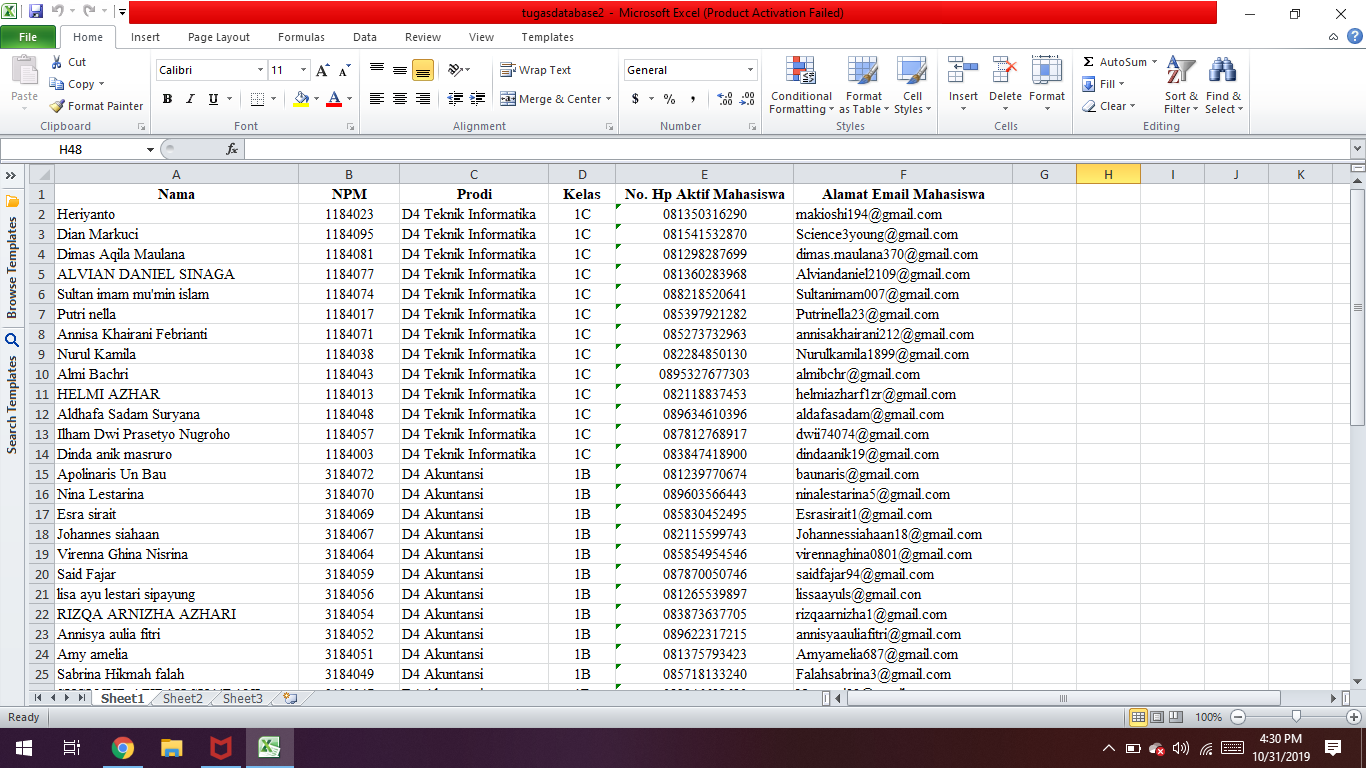
\includegraphics[scale=0.27]{figures/excel.png}
        \caption{Data Mahasiswa}
        \label{excel}
    \end{figure}
    \item Setelah itu anda masuk kedalam browser dan ketikkan laman apex.oracle.com lalu klik tombol sign in seperti pada gambar \ref{login1}
    \begin{figure}[!htbp]
        \centering
        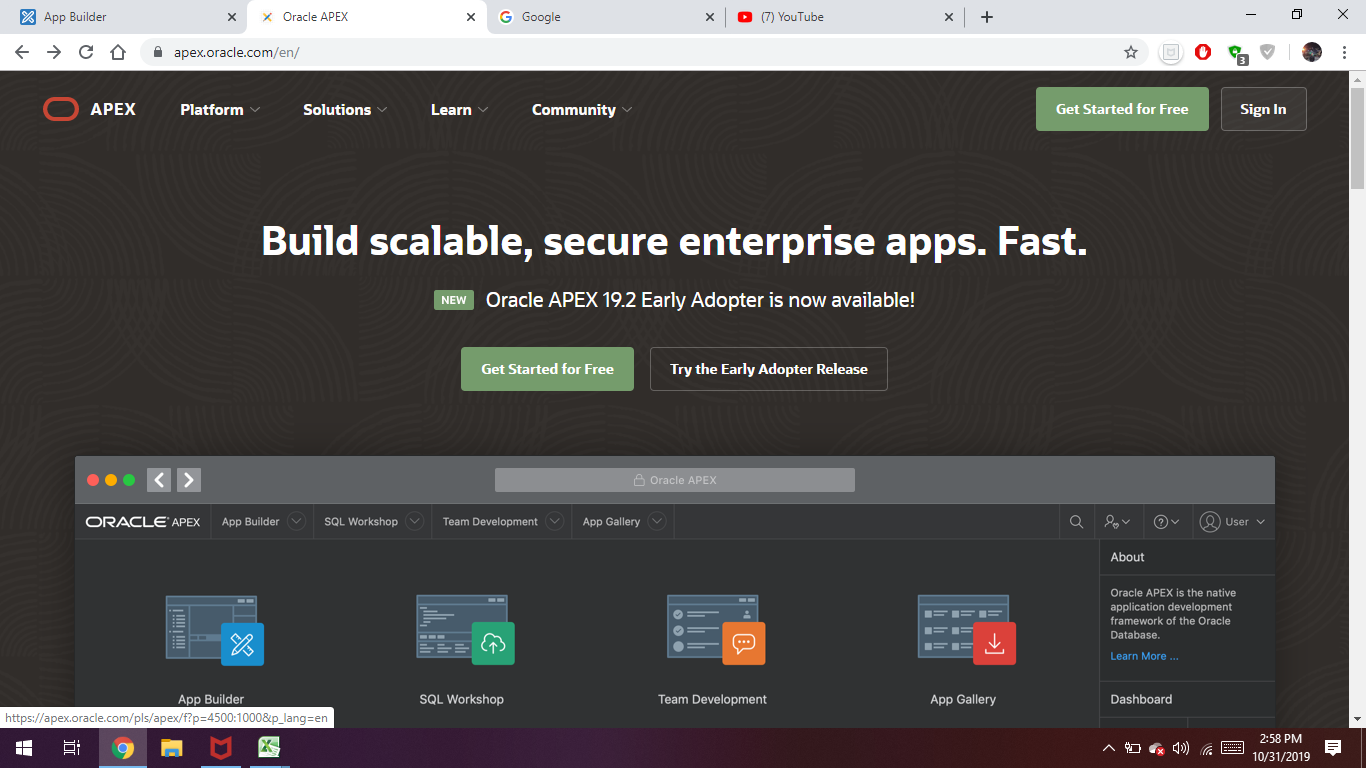
\includegraphics[scale=0.27]{figures/login1.png}
        \caption{Sign In Akun \textit{Oracle Apex}}
        \label{login1}
    \end{figure}
    \item Masukkan workspace, email, dan password kalian seperti pada gambar \ref{login2}
        \begin{figure}[!htbp]
        \centering
        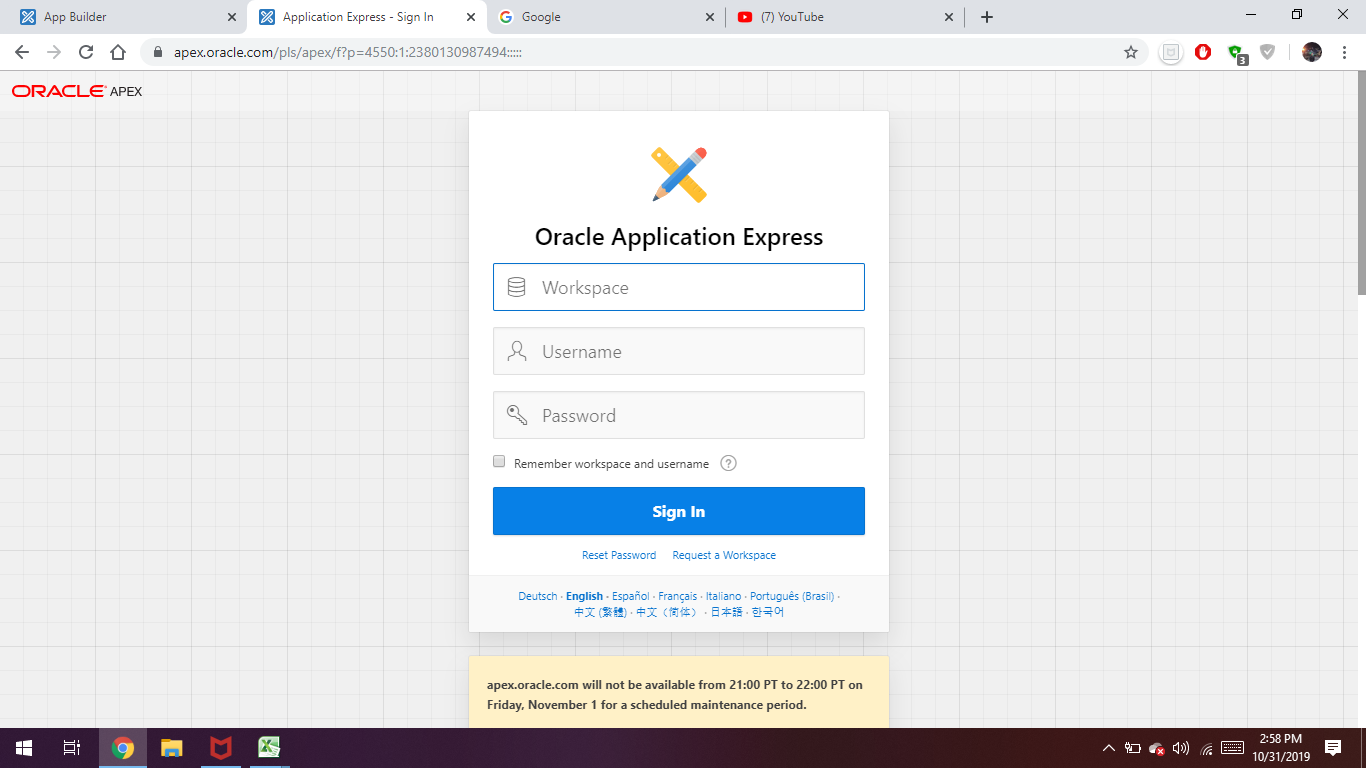
\includegraphics[scale=0.23]{figures/login2.png}
        \caption{Login Akun \textit{Oracle Apex}}
        \label{login2}
    \end{figure}
    \item Setelah masuk kedalam oracle apex klik App Builder seperti pada gambar \ref{aplikasi1} berikut
        \begin{figure}[!htbp]
        \centering
        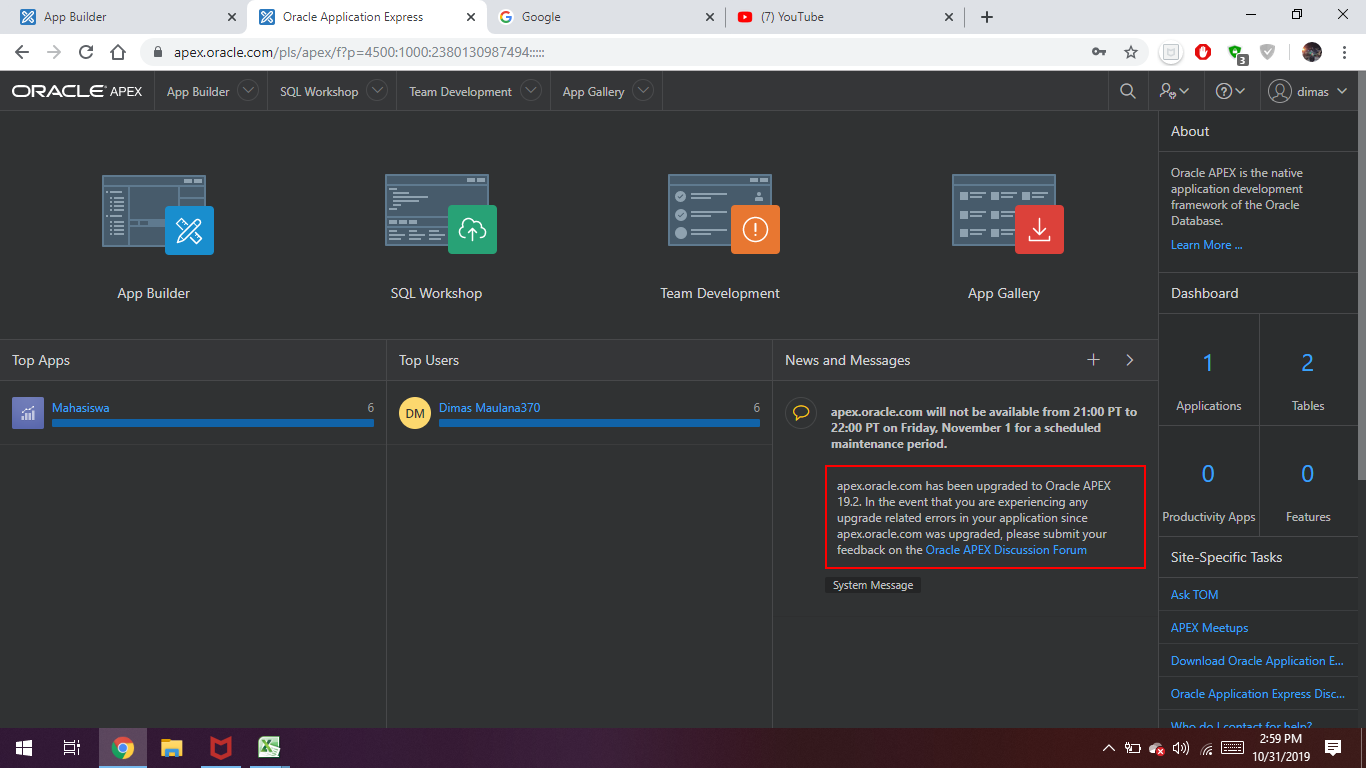
\includegraphics[scale=0.25]{figures/aplikasi1.png}
        \caption{Pembuatan Aplikasi}
        \label{aplikasi1}
    \end{figure}
    \item Lalu klik tombol create untuk membuat aplikasi tersebut seperti pada gambar \ref{aplikasi2}
            \begin{figure}[!htbp]
        \centering
        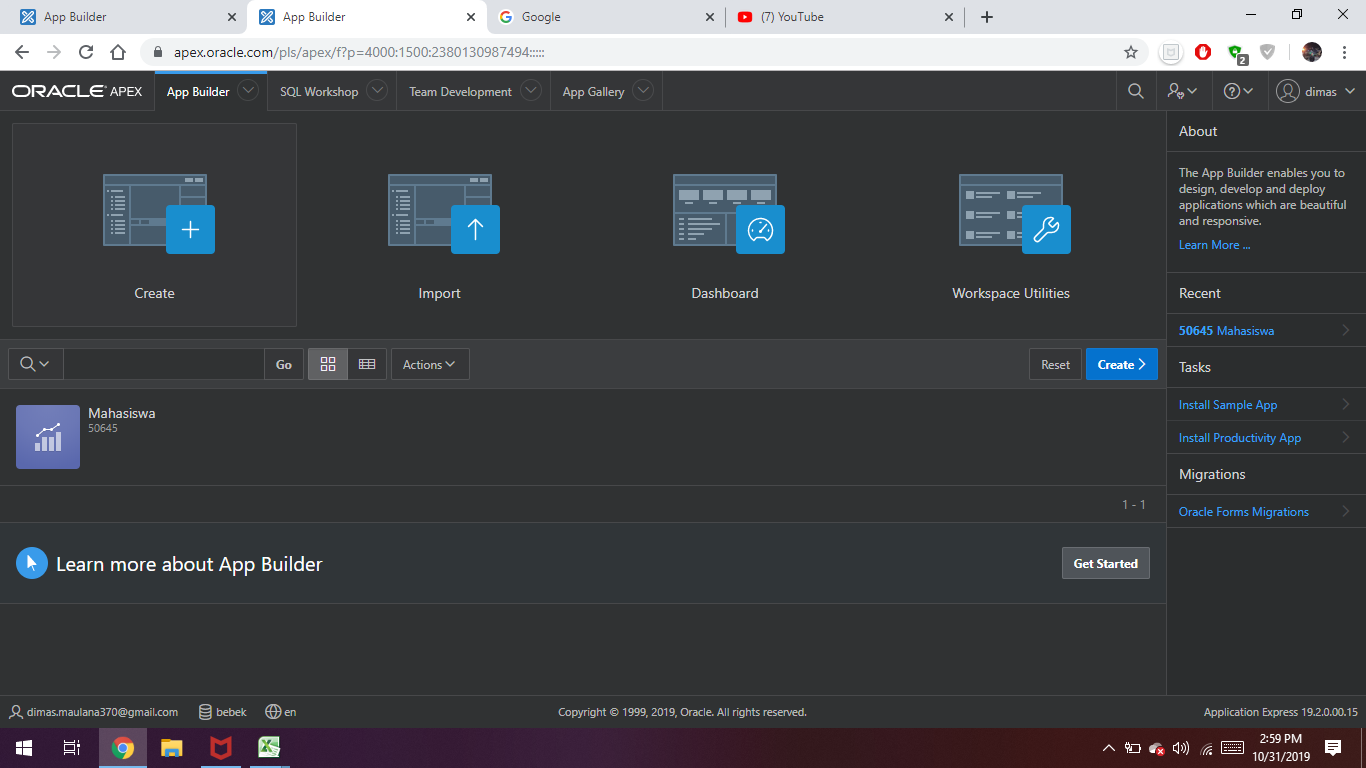
\includegraphics[scale=0.25]{figures/aplikasi2.png}
        \caption{Pembuatan Aplikasi}
        \label{aplikasi2}
    \end{figure}
    \item Setelah create maka ada 3 pilihan yaitu, new application, from a file,dan productivy app, kita pilih form a file karena sebelumnya kita sudah membuat data mahasiswa di microsoft excel seperti pada gambar \ref{aplikasi3}
            \begin{figure}[!htbp]
        \centering
        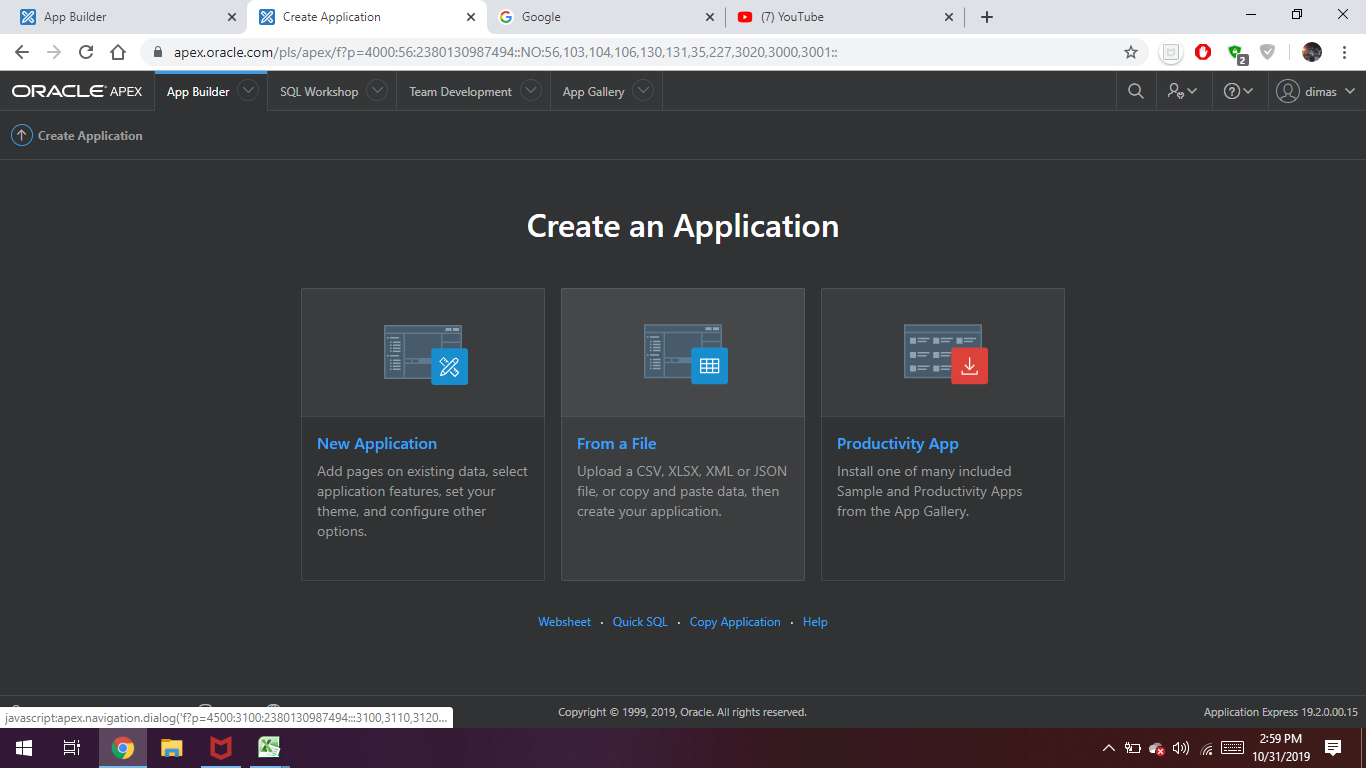
\includegraphics[scale=0.24]{figures/aplikasi3.png}
        \caption{Pembuatan Aplikasi}
        \label{aplikasi3}
    \end{figure}
    \item Masukkan file excel yang sudah kita buat tadi, bisa di drag atau klik choose file seperti pada gambar \ref{aplikasi4}
                \begin{figure}[!htbp]
        \centering
        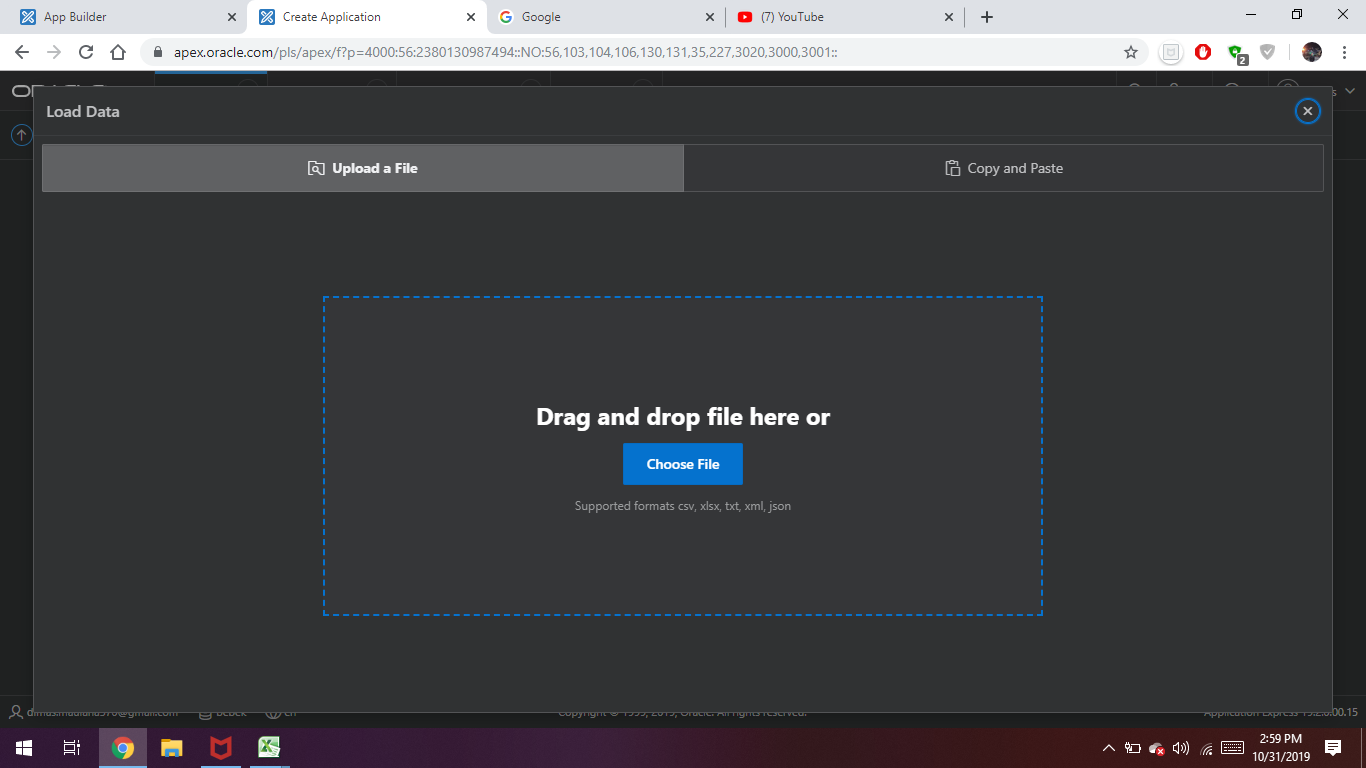
\includegraphics[scale=0.24]{figures/aplikasi4.png}
        \caption{Pembuatan Aplikasi}
        \label{aplikasi4}
    \end{figure}
    \item Setelah data excel dimasukkan maka akan beralih ke laman lain, anda sekalian disuruh untuk menamai tabel tersebut, disini saya menamai dengan DATA\_MAHASISWA lalu klik load data seperti pada gambar berikut \ref{aplikasi5}
    \begin{figure}[!htbp]
        \centering
        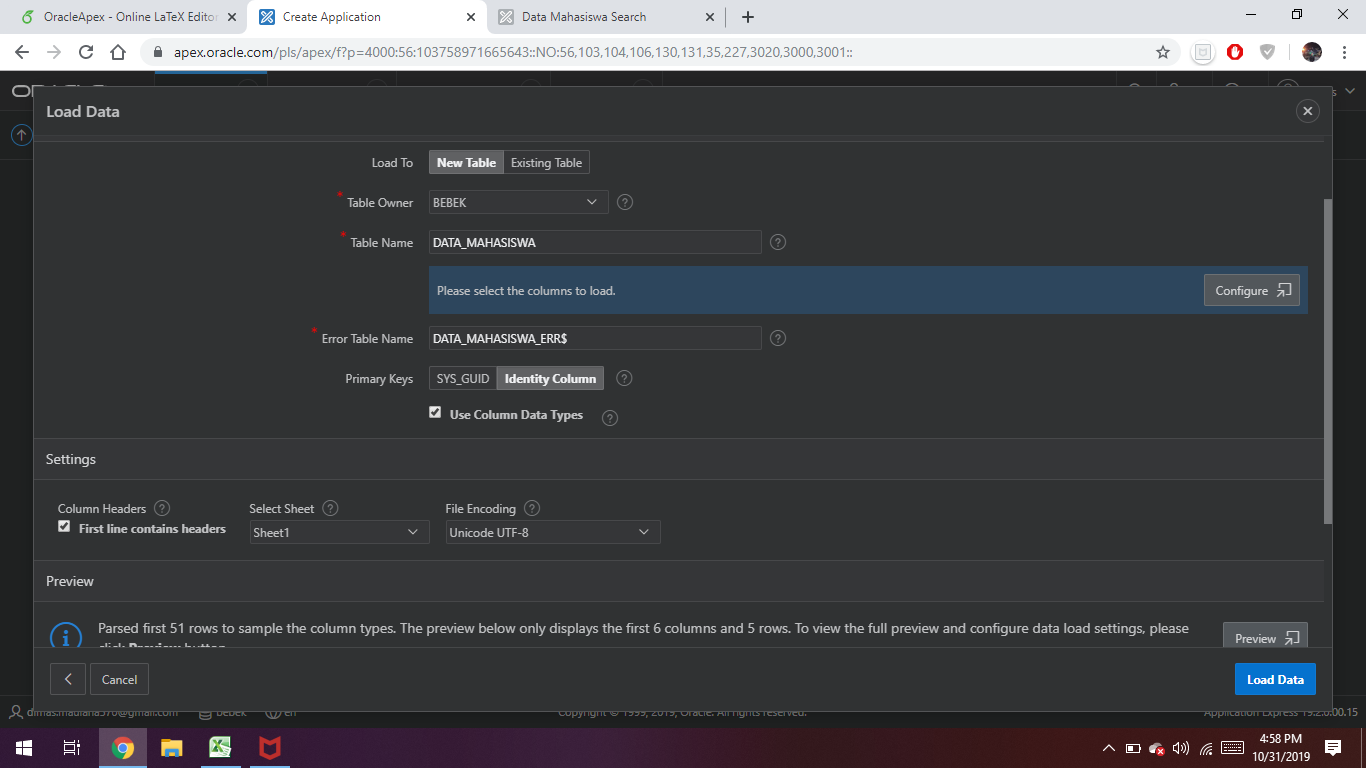
\includegraphics[scale=0.21]{figures/aplikasi5.png}
        \caption{Pembuatan Aplikasi}
        \label{aplikasi5}
    \end{figure}
    \item Kita disuruh untuk menunggu beberapa saat sampai data tersebut berhasil terunduh seperti pada gambar \ref{aplikasi6} lalu klik create application
    \begin{figure}[!htbp]
        \centering
        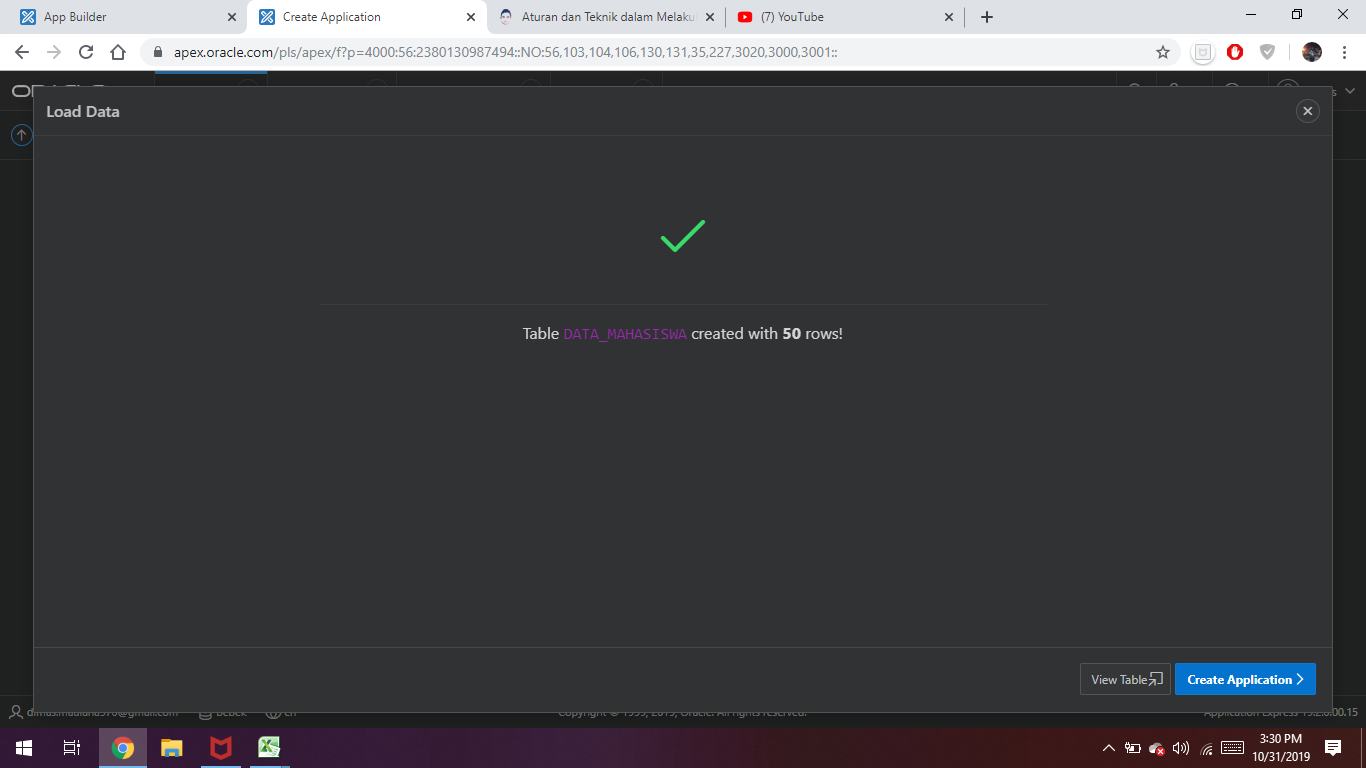
\includegraphics[scale=0.21]{figures/aplikasi6.png}
        \caption{Pembuatan Aplikasi}
        \label{aplikasi6}
    \end{figure}
    \item Setelah klik create application maka kita disuruh untuk mensetting lagi aplikasi tersebut apakah sudah benar atau belum, disini saya tidak mengubah apapun seperti pada gambar \ref{aplikasi7} lalu klik create application
    \begin{figure}[!htbp]
        \centering
        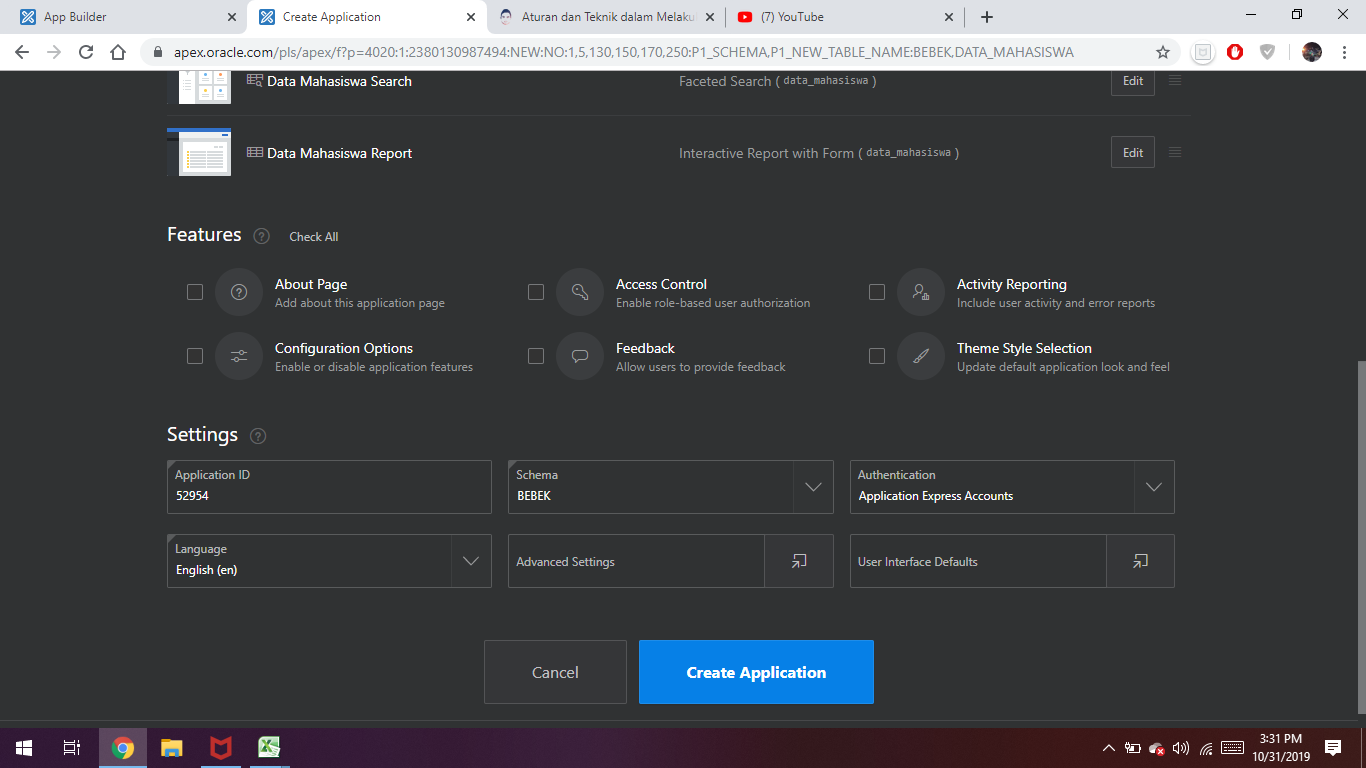
\includegraphics[scale=0.22]{figures/aplikasi7.png}
        \caption{Pembuatan Aplikasi}
        \label{aplikasi7}
    \end{figure}
    \item Setelah selesai membuat aplikasinya langsung saja kita klik tombol Run Application untuk melihat aplikasi yang sudah kita buat tadi seperti pada gambar \ref{aplikasi8}
    \begin{figure}[!htbp]
        \centering
        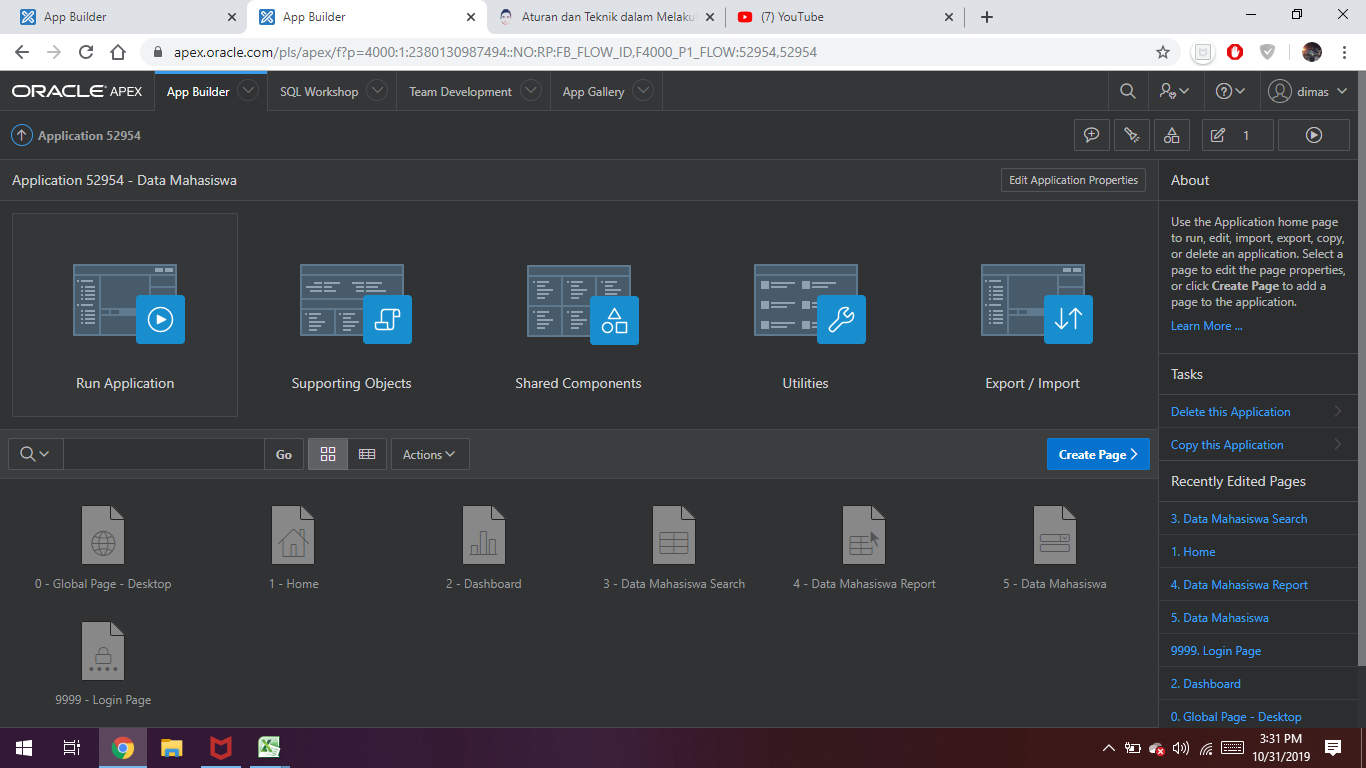
\includegraphics[scale=0.22]{figures/aplikasi8.png}
        \caption{Pembuatan Aplikasi}
        \label{aplikasi8}
    \end{figure}
    \item Kita dapat melihat aplikasi yang sudah kita buat tadi di oracle apex tabel tersebut sama seperti yang kita inputkan tadi yaitu Data Mahasiswa, disini kita bisa melihat grafik maupun data mahasiswa yang sudah kita inputkan tadi, didalam aplikasi ini sudah tersusun dengan rapi mulai dari prodi, kelas, npm, dan nomor hp mahasiswa tersebut seperti pada gambar \ref{aplikasi9}
    \begin{figure}[!htbp]
        \centering
        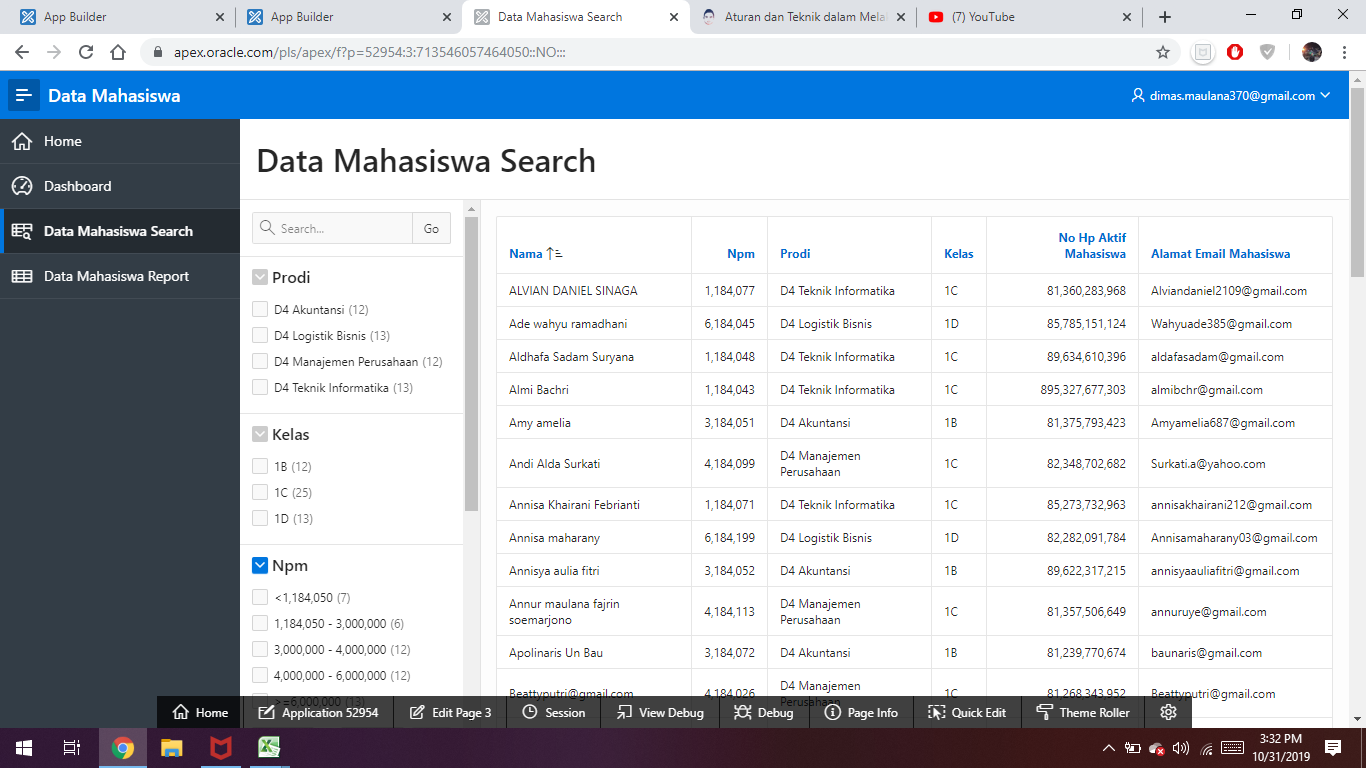
\includegraphics[scale=0.24]{figures/aplikasi9.png}
        \caption{Pembuatan Aplikasi}
        \label{aplikasi9}
    \end{figure}
    \end{figure}
    \item Jika kalian ingin mengubah kolom-kolom yang ada di tabel tersebut kalian bisa mengklik SQL workshop - Object Browser - Data\_Mahasiswa seperti pada gambar \ref{aplikasi11}
        \begin{figure}[!htbp]
        \centering
        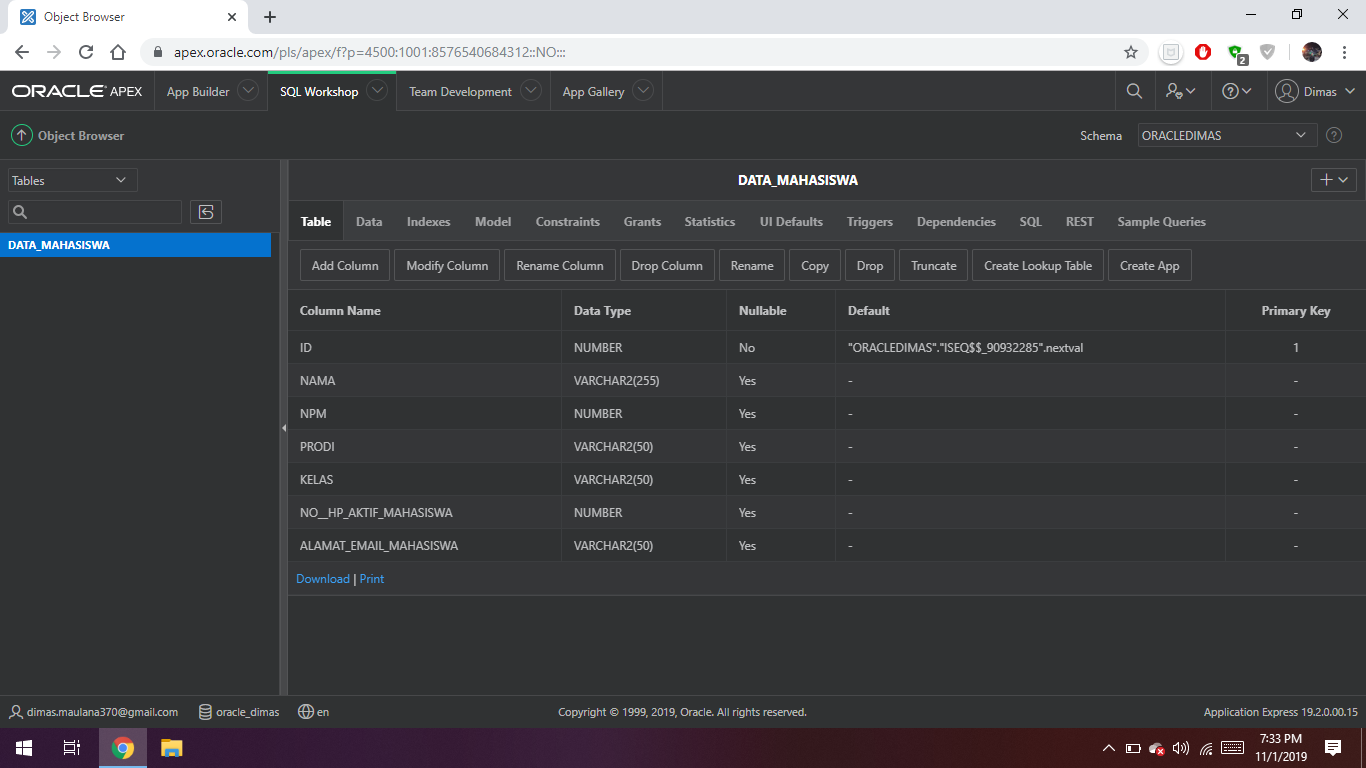
\includegraphics[scale=0.24]{figures/aplikasi11.png}
        \caption{Edit Tabel}
        \label{aplikasi11}
    \end{figure}
\end{itemize}

\section{ID PASSWORD ORACLE}
\par
Workspaces : ORACLE\_DIMAS
\par
Email : dimas.maulana370@gmail.com
\par
Password : redial24


\end{document}
